\documentclass[11pt]{article}
\usepackage[T1]{fontenc}
\usepackage[margin=1in]{geometry}
\usepackage{hyperref}
\usepackage{graphicx}
\usepackage{enumitem}
\usepackage{amsmath}

\title{ALCOR Timing Calibration Report}
\author{}
\date{}

\begin{document}
\maketitle

\section{Executive Summary}
This report documents the timing corrections developed for the ALCOR data, the calibration procedure used to derive them, and the results obtained so far. The goal is to reach sub-nanosecond timing resolution (target about 300 ps) by correcting fine-time non-linearities, time-walk, and channel-dependent offsets. The report is intentionally software-agnostic and focuses on the physics and analysis logic. 

The ALCOR V1 readout system (ALCOR) is used to read two silicon photomultiplier (SiPM) channels (ch 17 and ch 19),
specifically Onsemi 4$\times$4~mm$^2$ sensors from the Micro-J series,
using the fast output signal.

\section{Experimental Setup}
\subsection{Calibration setup}
The calibration uses a Hamamatsu picosecond light pulser (PLP-10 system) controlled by the C10196 controller. The PLP-10 provides laser pulses with typical width of about 70~ps full width at half maximum (FWHM) and repetition rates up to 100~MHz, with external trigger capability up to about 50~MHz.\footnote{Hamamatsu PLP-10 datasheet, \url{https://www.hamamatsu.com/content/dam/hamamatsu-photonics/sites/documents/99_SALES_LIBRARY/sys/SOCS0003E_PLP-10.pdf}.} During calibration it was operated at 100~kHz.

The light pulser illuminates two SiPMs from the onsemi Micro-J series (4$\times$4~mm$^2$ package, active area 3.93$\times$3.93~mm$^2$). The sensors provide a fast output obtained by capacitive coupling, used here for timing.\footnote{onsemi Micro-J series datasheet, \url{https://www.onsemi.com/download/data-sheet/pdf/microj-series-d.pdf}.}

\begin{figure}[ht]
  \centering
  \begin{minipage}{0.32\linewidth}
    \centering
    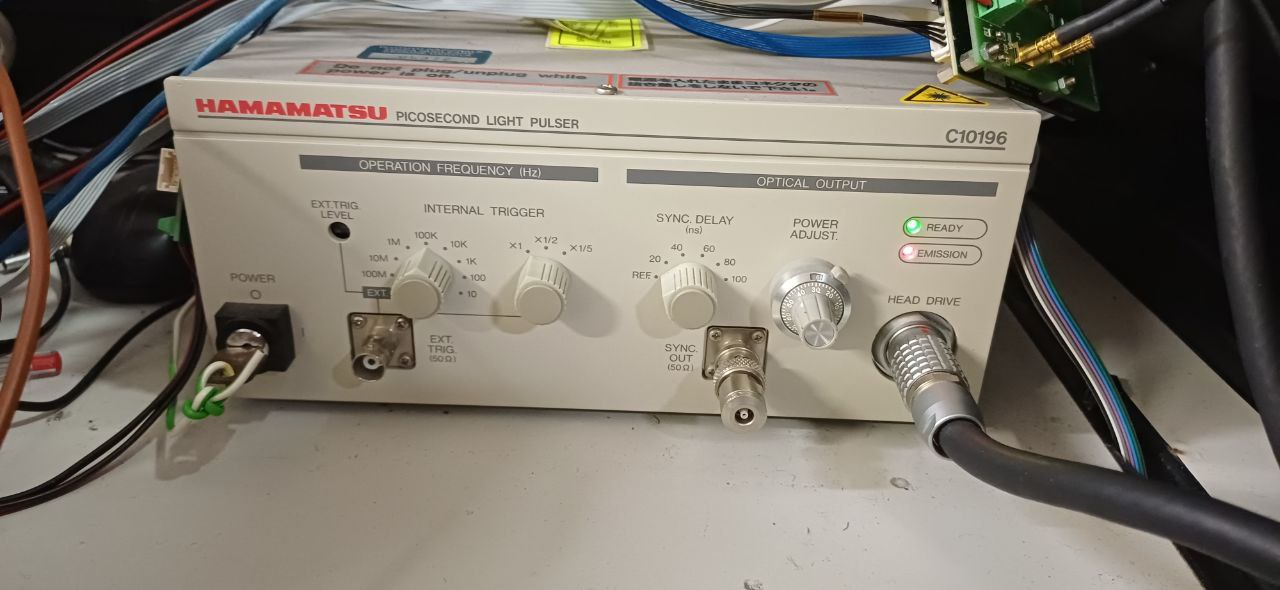
\includegraphics[width=\linewidth]{images/Laser_source.jpg}
    \vspace{2mm}
    \textbf{Laser source}
  \end{minipage}
  \hfill
  \begin{minipage}{0.32\linewidth}
    \centering
    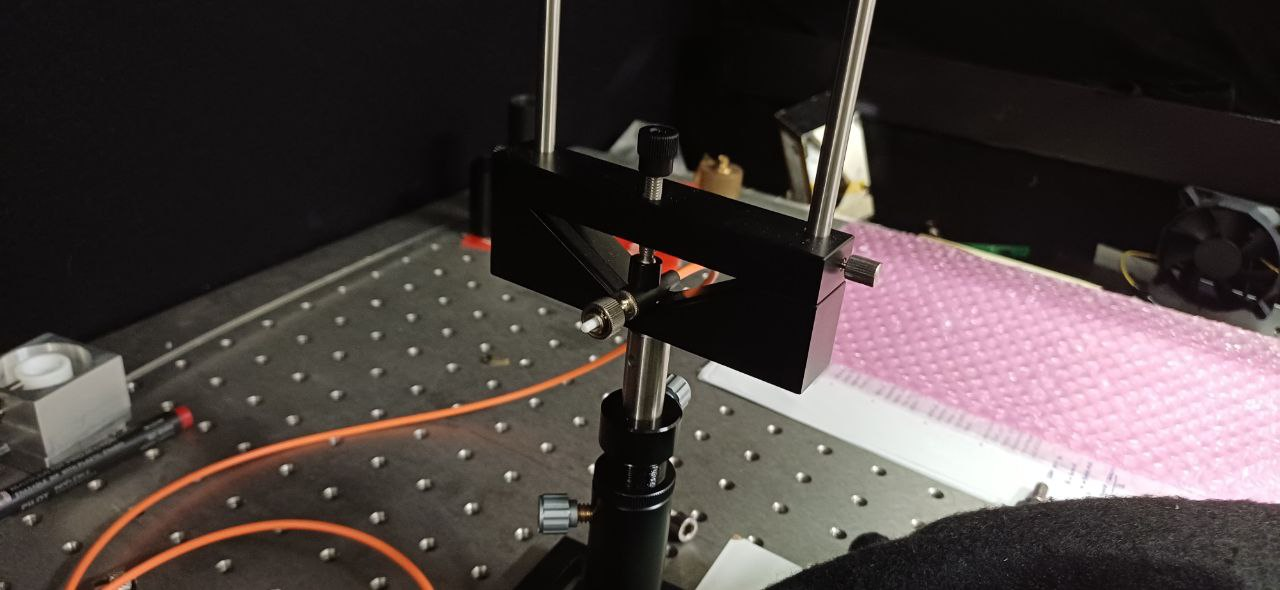
\includegraphics[width=\linewidth]{images/Laser_emitter.jpg}
    \vspace{2mm}
    \textbf{Emitter}
  \end{minipage}
  \hfill
  \begin{minipage}{0.32\linewidth}
    \centering
    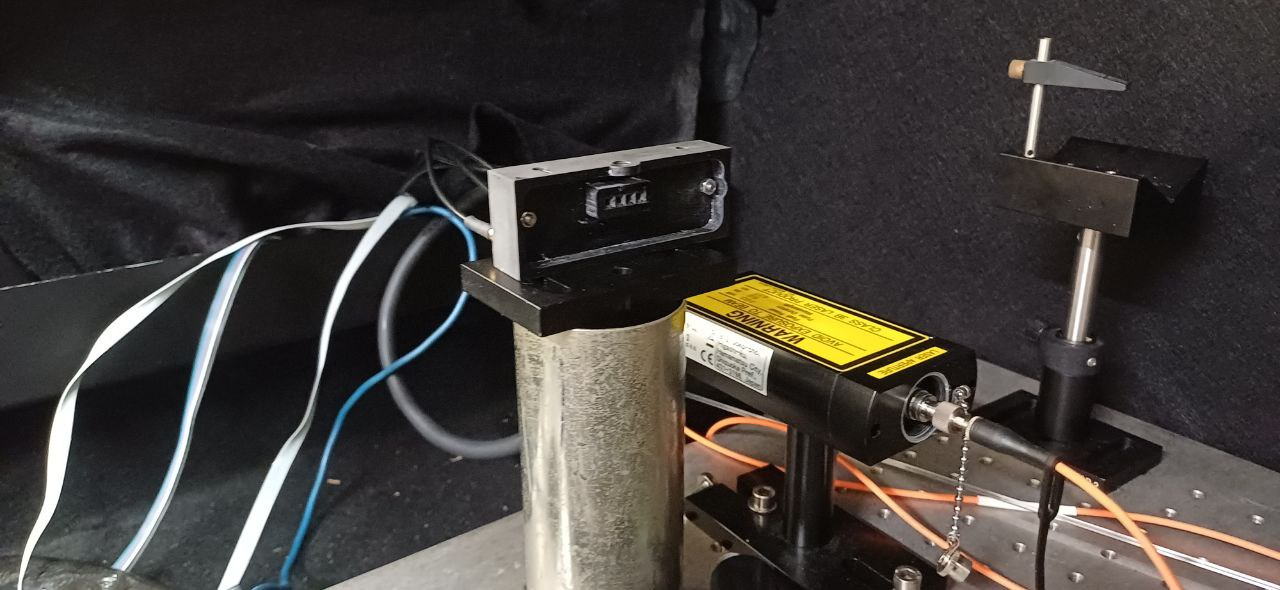
\includegraphics[width=\linewidth]{images/Sensori.jpg}
    \vspace{2mm}
    \textbf{SiPM sensors}
  \end{minipage}
  \caption{Calibration setup photographs.}
  \label{fig:setup_photos}
\end{figure}

\subsection{Scintillating fiber setup}
The second setup uses a 1~m scintillating fiber, with both ends coupled to the same two SiPMs.
A $^{90}$Sr beta source (10~kBq) is placed at the midpoint of the fiber to generate signals.


\section{Corrections Developed}

\subsection{Fine-time look-up table (LUT) (cumulative distribution function, CDF, linearization)}
The fine code exhibits local non-linearities: a simple linear min/max correction rescales the axis but cannot remove bin-to-bin distortions. In the calibration data the fine histogram shows a broad plateau with roll-off at the edges, but the mapping is not perfectly linear. The LUT corrects these local deviations and is therefore preferable to a linear mapping.

The LUT is appropriate when the arrival phase is effectively random with respect to the clock (e.g., dark counts or an unsynchronized laser). In that case the fine histogram is nearly flat with edge roll-off; if the fine distribution collapses to narrow peaks (phase locked), a LUT derived from those data would be biased and a phase-scan with a synchronized trigger is required instead.

For each TDC channel, let $b \in \{1,\dots,B\}$ be the fine-code bin (here $B=512$) and let $c_b$ be the bin counts. Define $N=\sum_{b=1}^{B} c_b$. The empirical CDF at bin $b$ is
\begin{align*}
F(b) &= \frac{1}{N}\left(\sum_{k \le b} c_k - \frac{1}{2}c_b\right),
\end{align*}
which corresponds to the CDF evaluated at the bin center. The fractional phase within a clock period is then
\begin{align*}
f(b) &= F(b) - \frac{1}{2}.
\end{align*}
Using this, the corrected timestamp is
\begin{align*}
t &= \left(R \cdot 2^{15} + C - f(b)\right)\,T, \\
T &= \frac{1000}{f_{\mathrm{clk}}}\;\mathrm{ns},
\end{align*}
where $R$ is the rollover count, $C$ is the coarse counter, and $f_{\mathrm{clk}}$ is the clock frequency in MHz.

The LUT is computed per TDC channel, so distinct channels are not mixed. Inter-channel timing corrections are applied symmetrically: the offset is split between the two channels so the alignment is to their mean time rather than choosing one channel as an absolute reference.

Differential non-linearity (DNL) quantifies the bin-to-bin deviation from a uniform population: \( \mathrm{DNL} = c_b/\langle c \rangle - 1 \). Integral non-linearity (INL) is the cumulative deviation from the ideal CDF: \( \mathrm{INL}(b) = F_{\mathrm{emp}}(b) - (b-0.5)/B \). Figures~\ref{fig:fine_validation_dnl} and~\ref{fig:fine_validation_inl} show that the LUT reduces both DNL and INL compared to the raw and linear corrections, indicating a more uniform fine-to-time mapping.

\begin{figure}[ht]
  \centering
  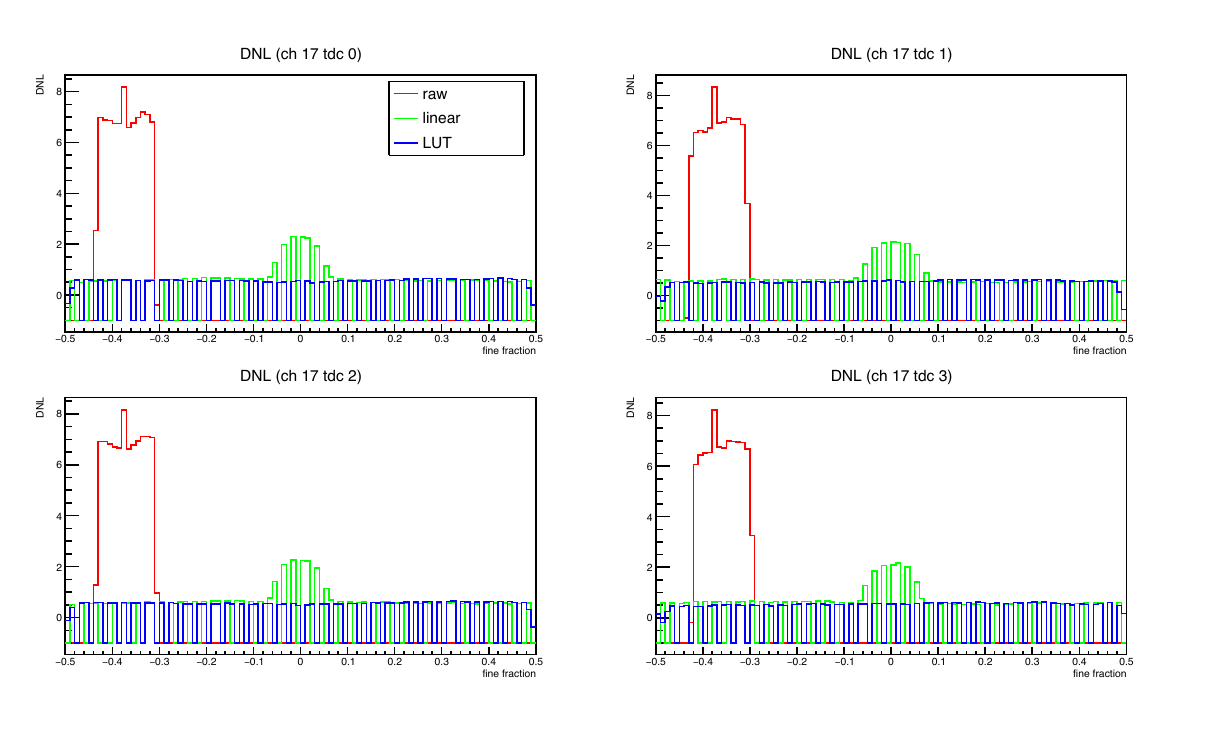
\includegraphics[width=0.95\linewidth]{figs/calibration_fine_validation_p15.png}
  \caption{DNL example (one channel). The plot compares raw, linear, and LUT‑corrected fine fractions; the LUT curve is closest to the ideal uniform response.}
  \label{fig:fine_validation_dnl}
\end{figure}

\begin{figure}[ht]
  \centering
  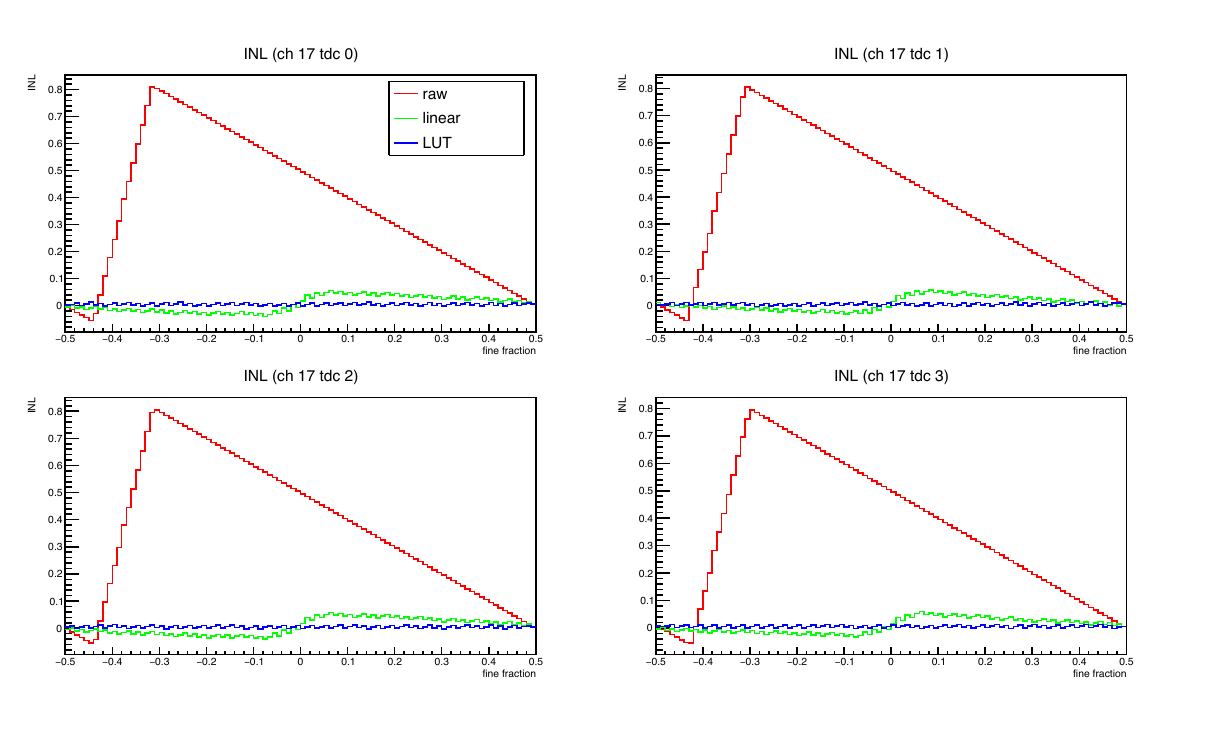
\includegraphics[width=0.95\linewidth]{figs/calibration_fine_validation_p16.png}
  \caption{INL example (one channel). The LUT strongly reduces the cumulative non‑linearity compared to the linear correction.}
  \label{fig:fine_validation_inl}
\end{figure}

\subsection{Time-walk (Time-over-Threshold, ToT, dependent correction)}
Leading-edge timing depends on pulse amplitude. The Time-over-Threshold (ToT) provides a proxy for pulse amplitude, so we correct timing as a function of ToT.

\begin{itemize}[leftmargin=*]
  \item Use a reference channel and build $\Delta t$ vs ToT for each channel.
  \item Only leading edges are corrected; ToT is computed from the trailing edge association.
  \item A median per ToT bin is used to reduce sensitivity to tails and outliers.
  \item The correction is derived iteratively:
  \begin{enumerate}[leftmargin=*]
    \item Compute $\Delta t(\mathrm{ToT})$ from raw times.
    \item Apply the correction and recompute $\Delta t(\mathrm{ToT})$.
    \item Use the refined curve as the final correction.
  \end{enumerate}
  \item A symmetric mode splits the correction between the reference and the channel so the reference is not artificially fixed.
\end{itemize}

For each leading hit:
\begin{align*}
 t_{\mathrm{lead, corrected}} = t_{\mathrm{lead}} - \mathrm{Correction}(\mathrm{ToT})
\end{align*}

\subsection{Channel-dependent offsets}
After ToT correction, a residual timing offset may remain due to fixed channel delays.

\begin{itemize}[leftmargin=*]
  \item Build a residual $\Delta t$ distribution (after ToT correction) per channel.
  \item Fit a Gaussian and take the mean as the offset.
  \item Offsets are also applied symmetrically in the reference-split mode.
\end{itemize}

\section{Calibration Procedure}

\subsection{Input data}
\begin{itemize}[leftmargin=*]
  \item Calibration run: Laser/impulse data (\texttt{data/calibration}).
  \item Validation run: Physics reference data (\texttt{data/golden\_run}).
\end{itemize}

\subsection{Steps}
\begin{enumerate}[leftmargin=*]
  \item \textbf{Fine LUT calibration (CDF linearization)}
    \begin{itemize}
      \item Build fine histograms for each physical TDC.
      \item Extract min/max and LUT per TDC.
    \end{itemize}
  \item \textbf{Time-walk calibration (ToT)}
    \begin{itemize}
      \item Use the calibration run with a reference channel (currently ch 19).
      \item Compute $\Delta t(\mathrm{ToT})$ per channel using the median per bin.
      \item Iterate once to refine the correction.
    \end{itemize}
  \item \textbf{Offset calibration}
    \begin{itemize}
      \item After ToT correction, fit residual $\Delta t$ to extract per-channel offsets.
    \end{itemize}
  \item \textbf{Validation}
    \begin{itemize}
      \item Apply the full calibration set to the golden run.
      \item Compare coincidence peak width (FWHM or $\sigma$) and stability to the uncorrected case.
    \end{itemize}
\end{enumerate}

\section{Results Obtained (Current)}

\subsection{Fine LUT}
The LUT produces a near-uniform fine-fraction distribution as expected from the CDF construction. Intrinsic and cross-validation metrics indicate improved uniformity (details to be added with plots).

\subsection{Time-walk correction magnitude}
The ToT-based correction is of order 2--3 ns in amplitude for channels 17/19, consistent with the expected size of time-walk. This is a large correction compared to the 300 ps target, but it is the offset that must be removed to reach that resolution.

\subsection{Symmetric correction}
In symmetric mode, the reference channel is also corrected to avoid biasing the timing scale of the reference alone.
\subsection{Laser calibration comparison (page 3)}
Figure~\ref{fig:laser_calib_page3} compares page~3 of the calibration runs without and with the full calibration chain. This illustrates the tightening of the laser-based coincidence measurements after applying the corrections.

\begin{figure}[ht]
  \centering
  \begin{minipage}{0.49\linewidth}
    \centering
    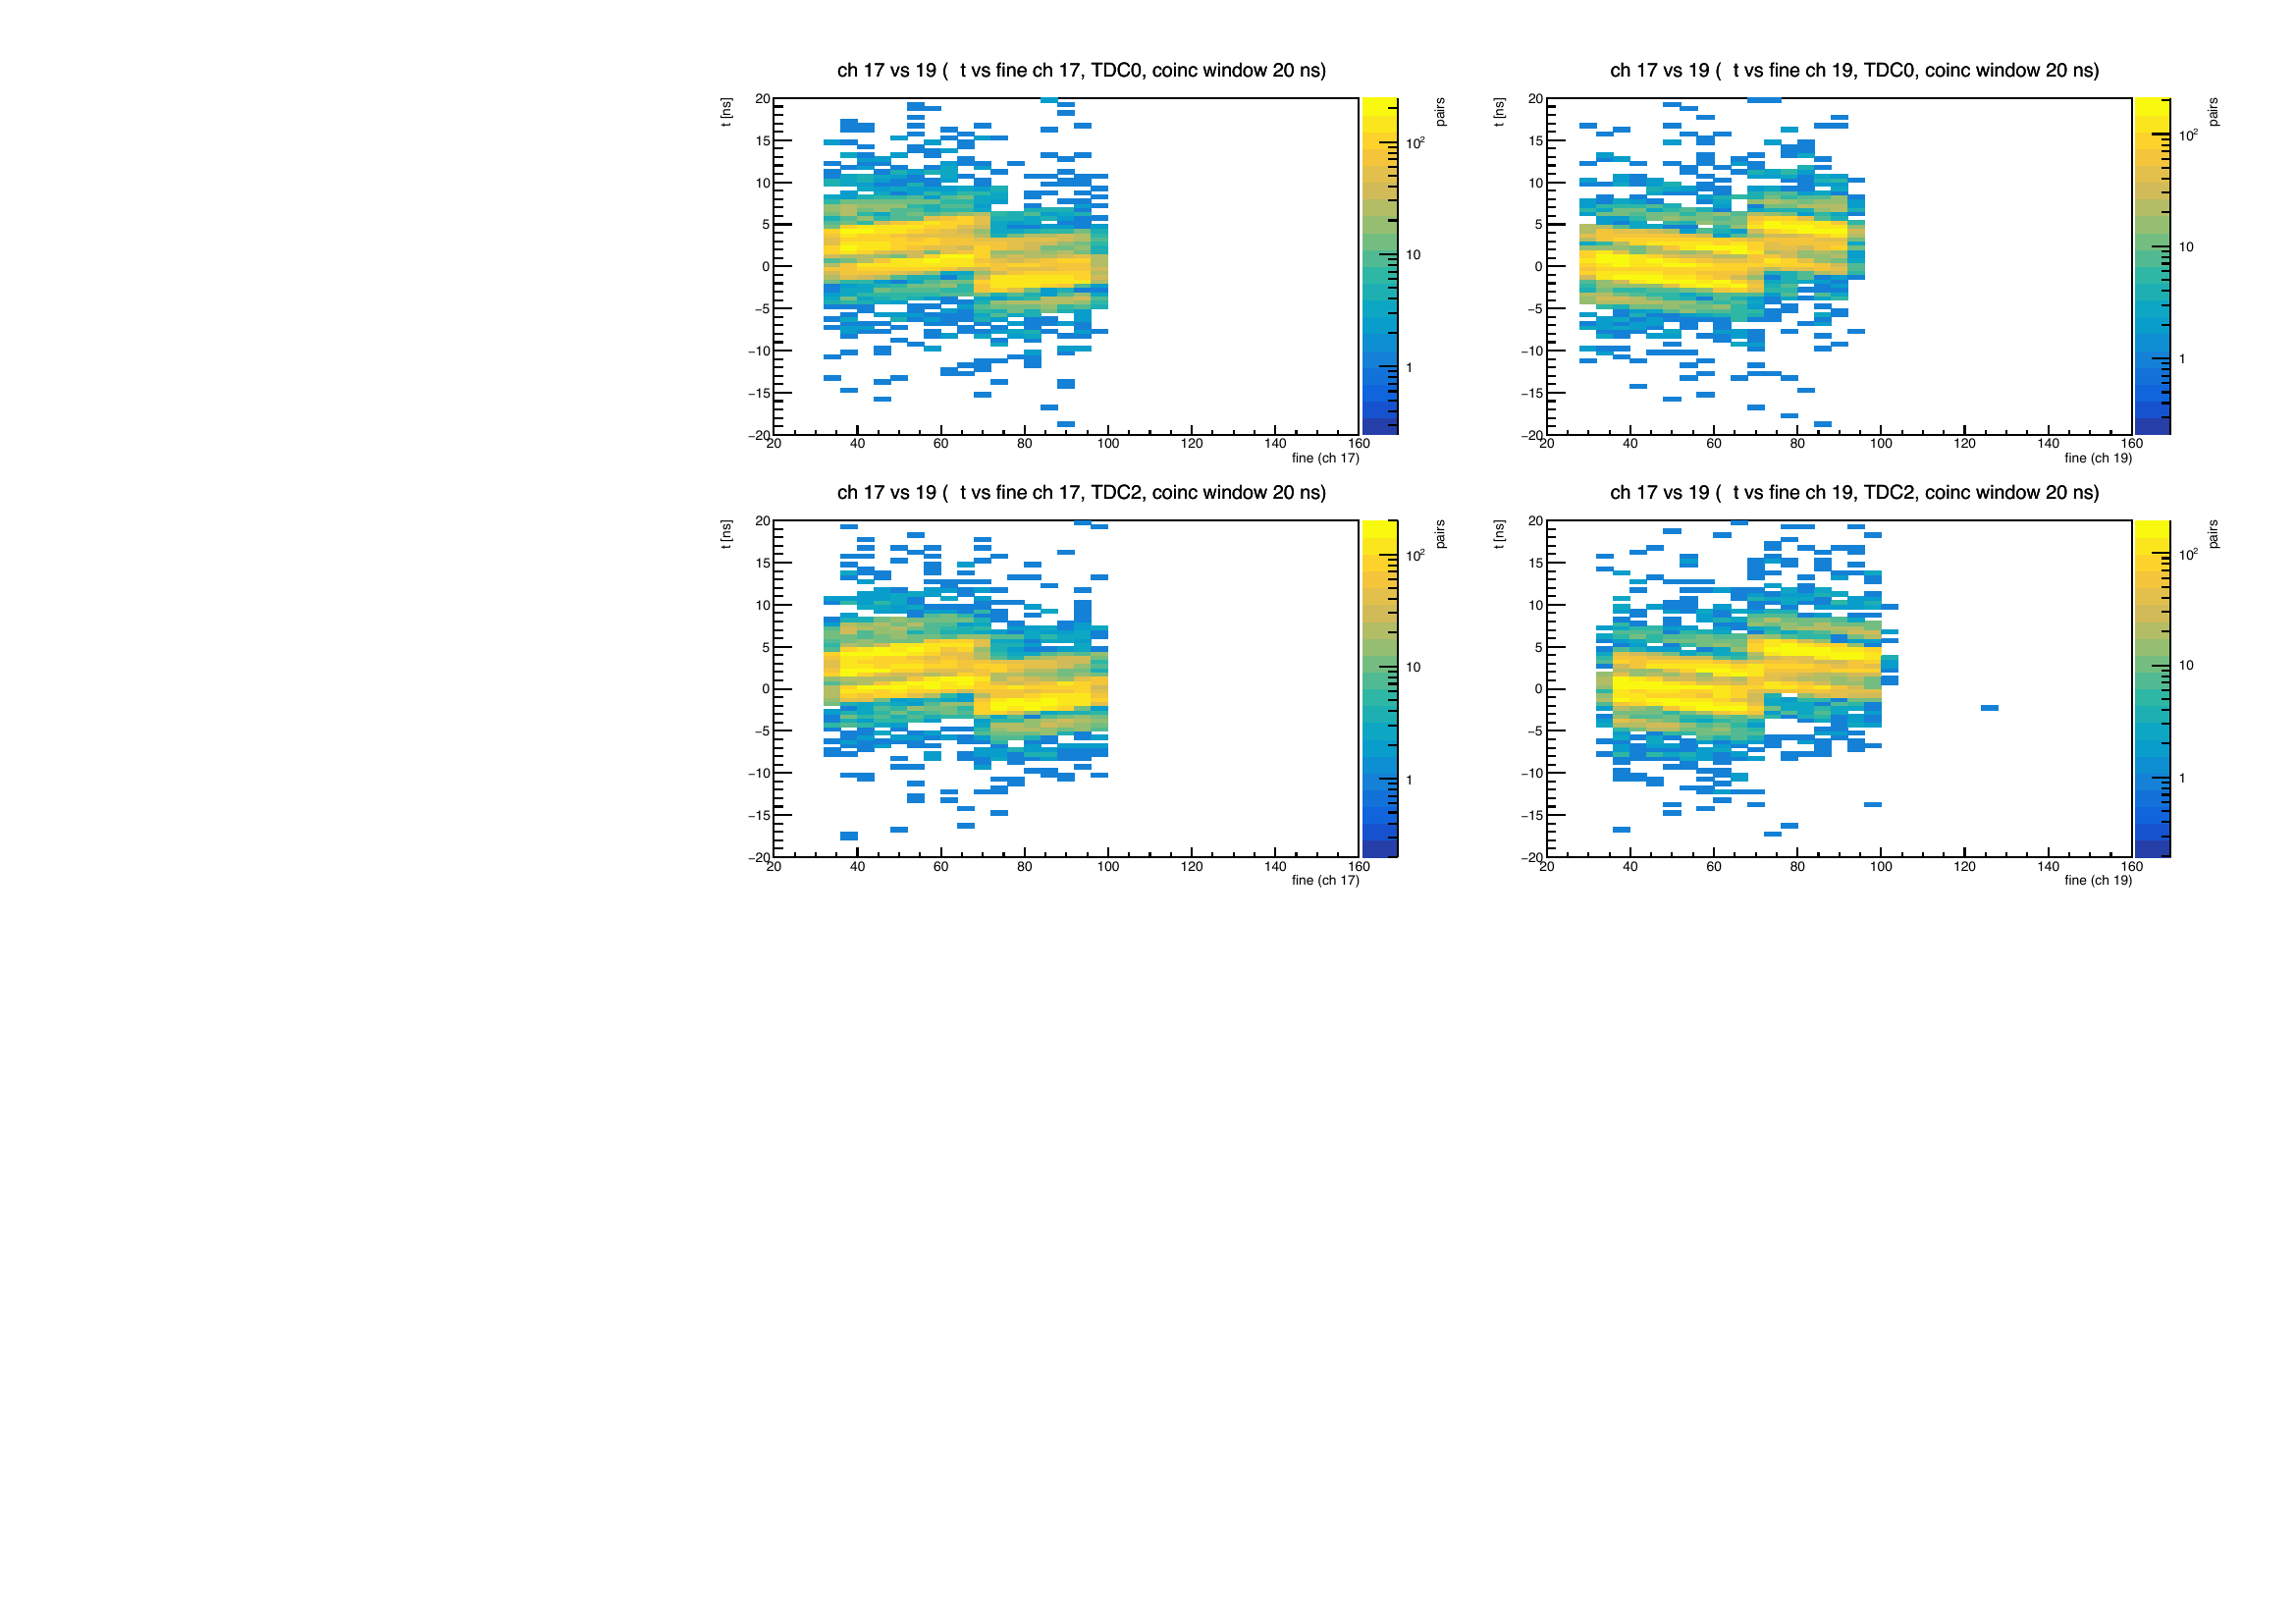
\includegraphics[width=\linewidth]{figs/calibration_no_calib_page3-03.png}
    \vspace{2mm}
    \textbf{No calibration}
  \end{minipage}
  \hfill
  \begin{minipage}{0.49\linewidth}
    \centering
    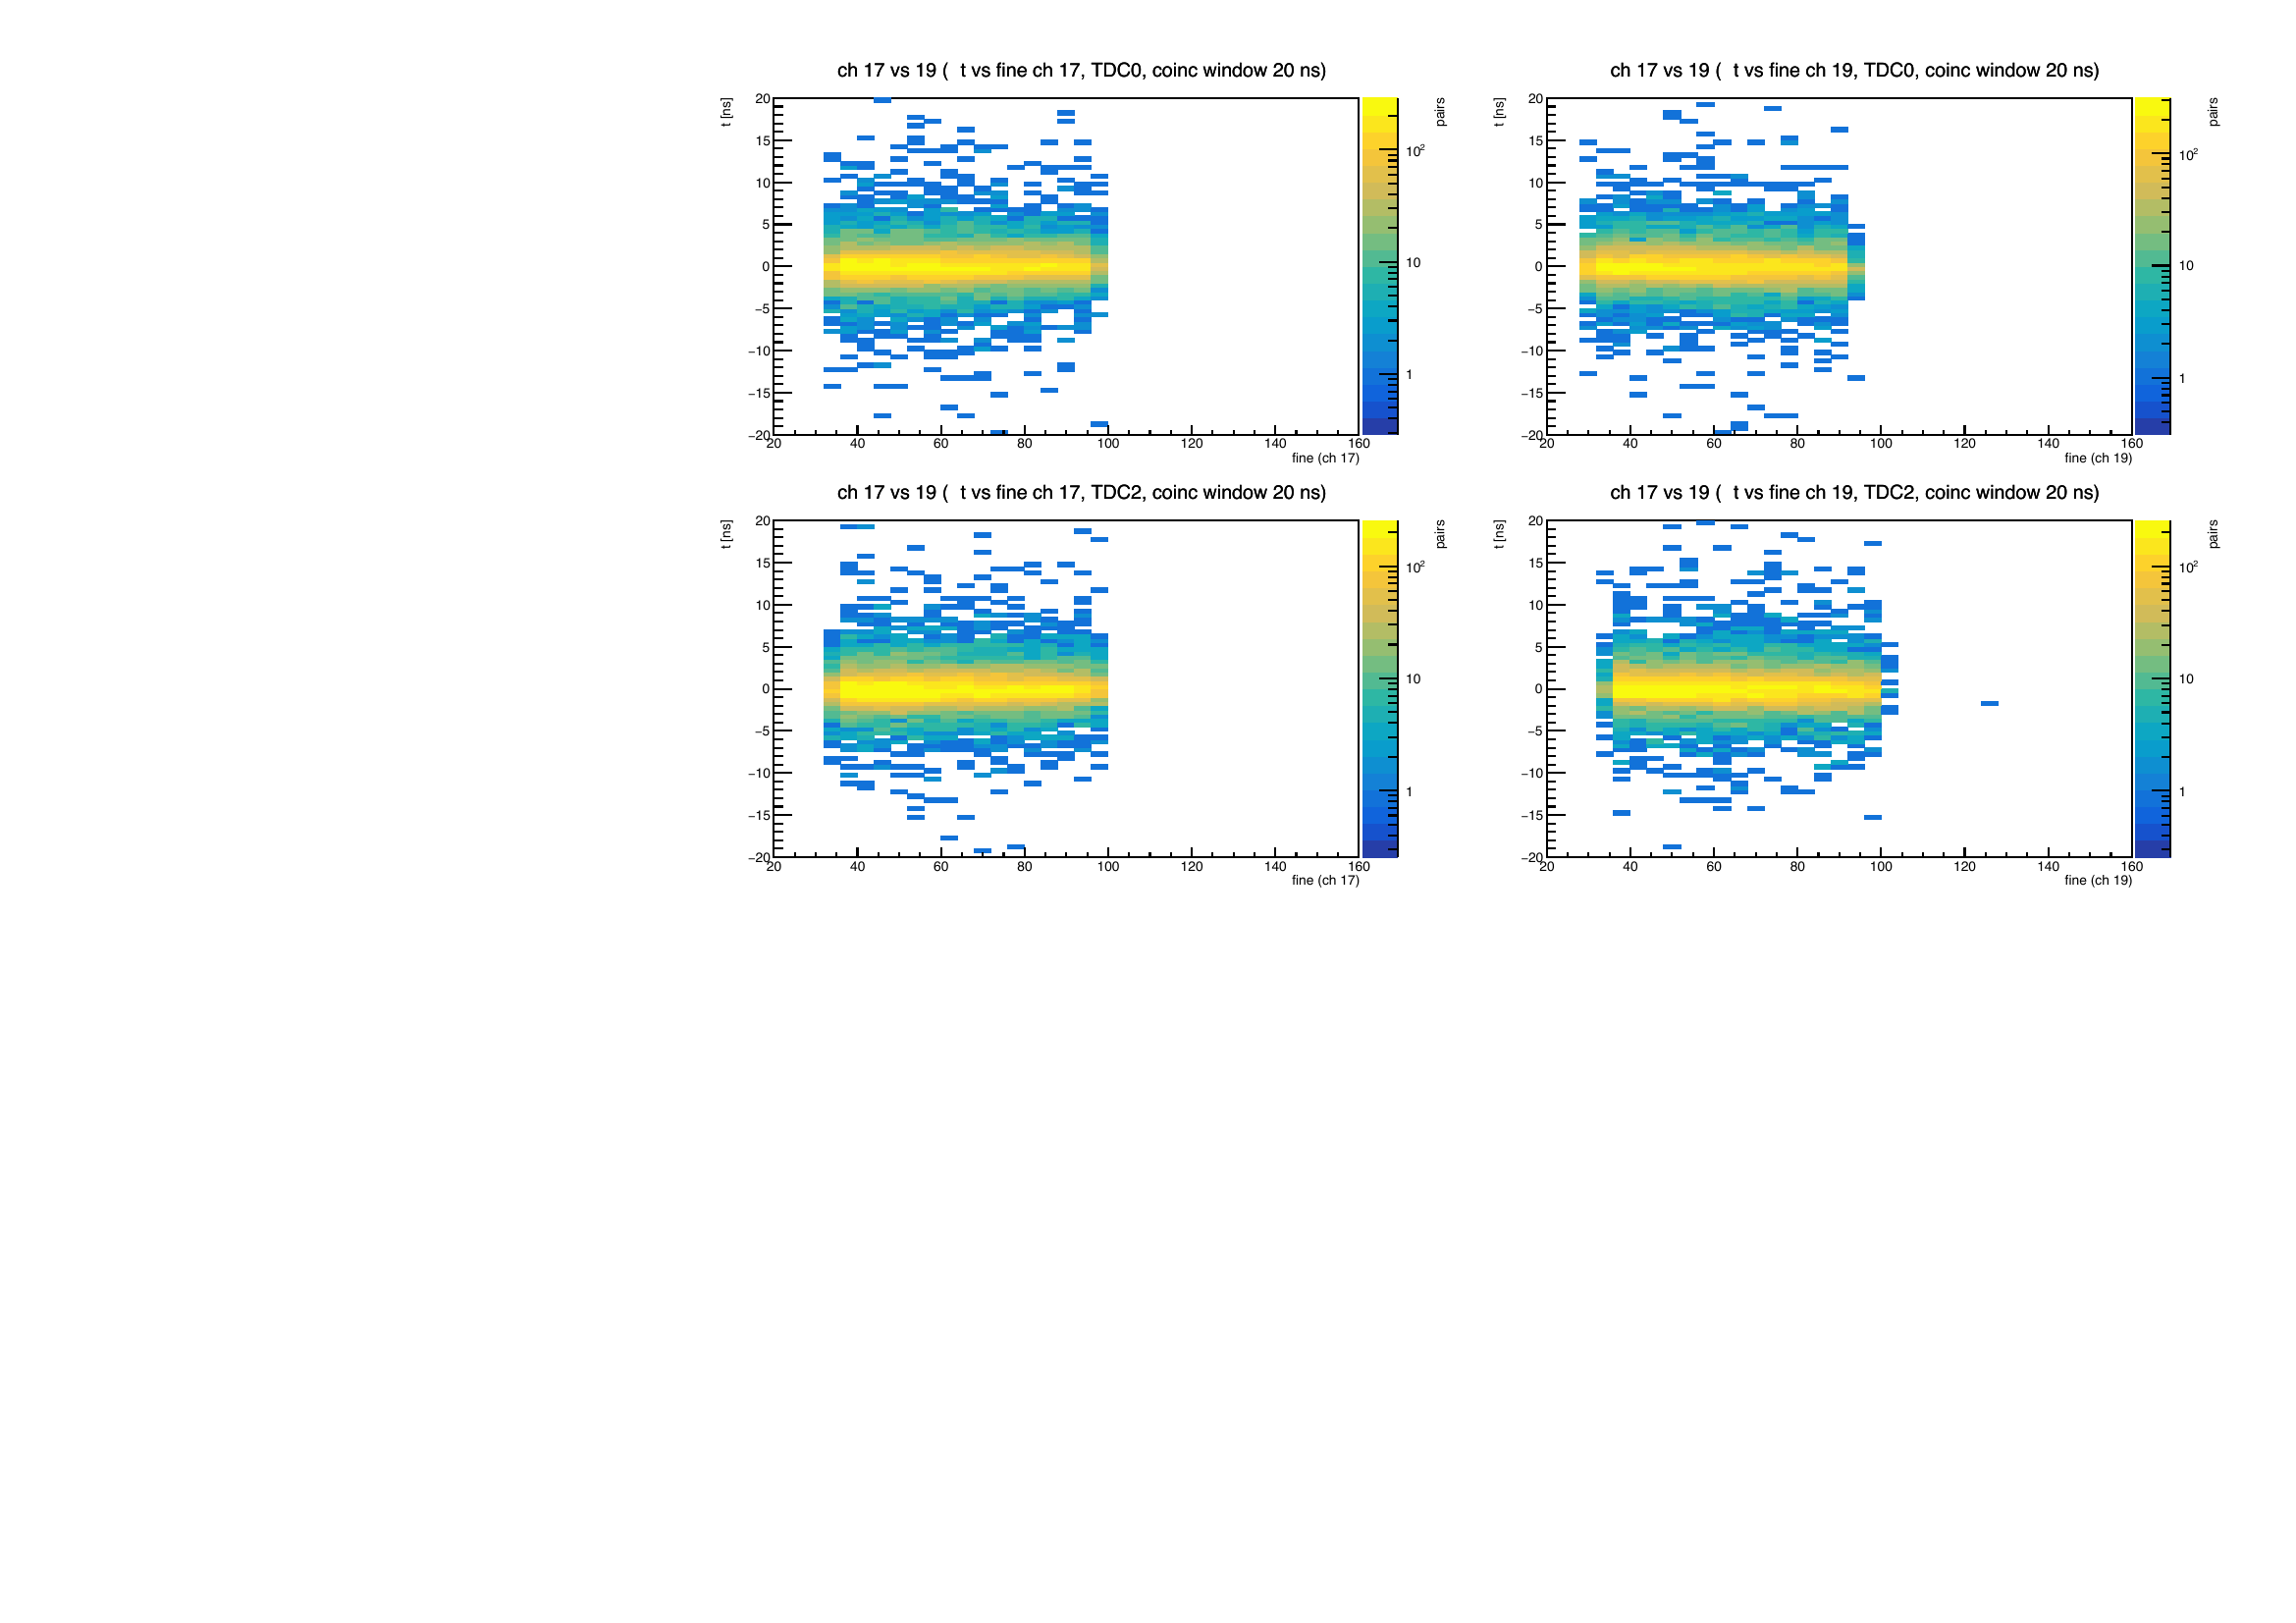
\includegraphics[width=\linewidth]{figs/calibration_with_calib_page3-03.png}
    \vspace{2mm}
    \textbf{With calibration}
  \end{minipage}
  \caption{Calibration run (laser) comparison using page 3.}
  \label{fig:laser_calib_page3}
\end{figure}

\section{Notes and Assumptions}
\begin{itemize}[leftmargin=*]
  \item The ToT correction is applied only when a valid trailing edge exists (ToT is defined).
  \item Coincidence matching uses nearest hits within a time window; tight windows reduce accidental biases.
  \item The reference channel selection affects the calibration; symmetric correction mitigates this.
\end{itemize}

\end{document}
